\documentclass[12pt]{article}

\usepackage[spanish]{babel} % Remove this line if you want English language support
\usepackage[hyperindex]{hyperref}
\usepackage{graphicx}
\usepackage{enumitem}
\usepackage{subfiles} % Best loaded last in the preamble

\addto\captionsspanish{\renewcommand{\contentsname}{Tabla de Contenidos}}

\begin{document}

\title{\textbf{FIUBAKKA} \\ \large \textbf{Juego multijugador online con Akka}}
\author{
    Rolando, Marcos
    \and
    Soriano, Iván
    \and
    Raveszani, Nicole
    \and
    Scaccheri Cassanello, Franco
    \and
    Deymonnaz, Pablo
}
\date{\today}

\maketitle % Prints the title, author, and date

\thispagestyle{empty}

\begin{figure}[htbp]
    \centering
    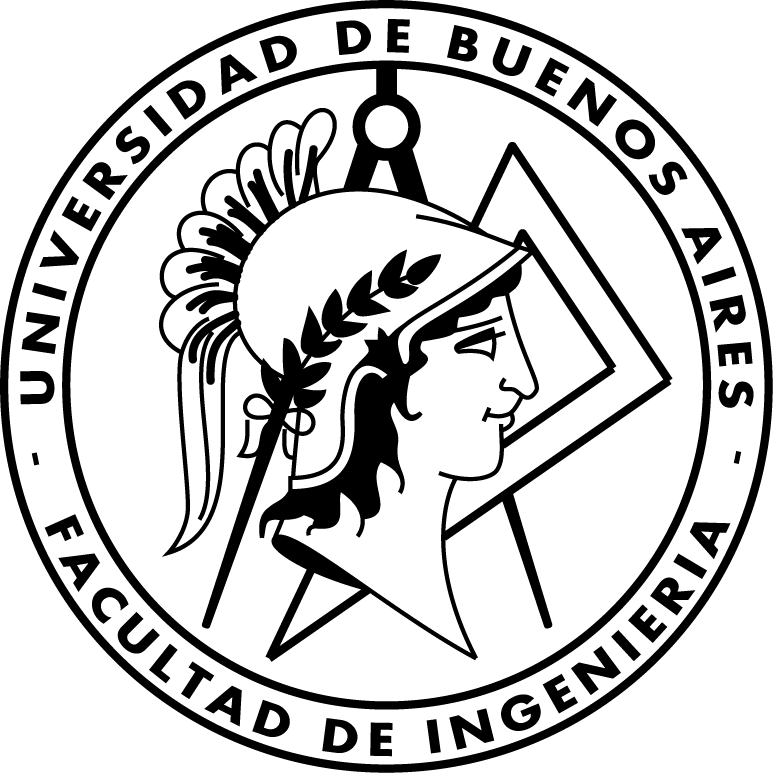
\includegraphics[width=0.5\textwidth]{../assets/fiuba-logo.png}
\end{figure}
\begin{figure}[htbp]
    \centering
    
\includegraphics[width=0.5\textwidth]{../assets/akka-toolkit-logo.png}
\end{figure}

\newpage
\thispagestyle{empty}
\tableofcontents
\newpage

\setcounter{page}{1} % Reset page counter to 1

\section{Resumen}

\subfile{resumen.tex}

\section{Palabras clave}

\subfile{palabras_clave.tex}

\newpage

\vspace{5mm} %5mm vertical space

\section{Abstract}

\subfile{abstract.tex}

\section{Keywords}

\subfile{keywords.tex}

\newpage

\section{Introducción}

\subfile{introduction.tex}

\section{Estado del Arte}

\subfile{state_of_art.tex}

\section{Problema detectado y/o faltante}

\subfile{problem.tex}

\section{Solución implementada}

\subfile{solution.tex}

\section{Metofología aplicada}

\subfile{methodology.tex}

\section{Experimentación y/o validación}

\subfile{validation.tex}

\section{Cronograma de las actividades realizadas}

\subfile{chronogram.tex}

\section{Riesgos materializados y Lecciones aprendidas}

\subfile{lessons.tex}

\section{Conclusiones}

\subfile{conclusions.tex}

\section{Referencias}

\subfile{references.tex}

\section{Anexos}

\subfile{appendix.tex}


\end{document}
